\section{Architektur}\label{sec:architecure}
Nun gilt es das in Kapitel \ref{sec:konzept} vorgestellte Konzept umzusetzen. Dazu wurde eine Architektur für einen Sprachassistenten entwickelt, welche in Abbildung \ref{fig:infrastruktur-overview} zu sehen ist. Diese Architektur bietet mehr Privatsphäre und ist unterteilt in drei Hauptmodule: Die Mobile App, das Repository und die Cloud. Dabei existiert das Modul \glqq Speech Processing\grqq{} in der Mobilen App und in der Cloud. In der Mobilen App werden einfache Sprachverarbeitungsprozesse wie beispielsweise das Aufnehmen bzw. die Wiedergabe eines Audiofiles implementiert. Ressourcenintensive Sprachverarbeitungsprozesse, wie beispielsweise die Umwandlung von Sprache zu Text, werden in die Cloud ausgelagert. Im Folgenden sind die drei Hauptmodule genauer beschrieben.
\begin{figure}[h!]
	\centering
	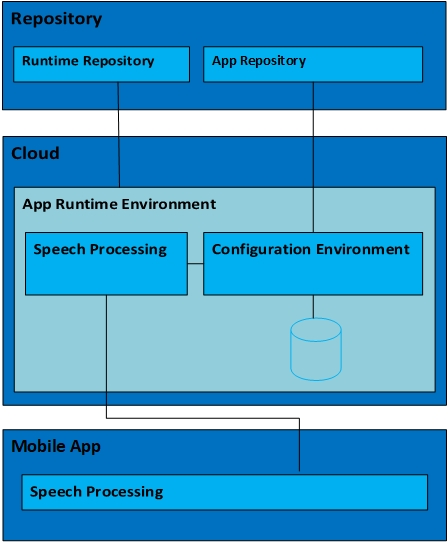
\includegraphics[width=0.8\linewidth]{Picture/Infrastruktur-Overview.jpg}
	\caption[Architekturübersicht]{Architekturübersicht}
	\label{fig:infrastruktur-overview}
\end{figure}

\subsection{Mobile App}
Die Mobile App ist die Schnittstelle zum Nutzer und wie Abbildung \ref{fig:infrastruktur-app} zeigt, hat diese drei Module:

\begin{itemize}
	\item \textsl{Speech Recording:} Aufnehmen und streamen der Eingabe eines Nutzers an die Cloud.
	\item \textsl{Speech Playback:} Abspielen eines Streams, der von der Cloud erzeugt wurde, an den Nutzer.
	\item \textsl{Hotword Detection:} Die Mobile App soll nicht ununterbrochen die Eingabe des Nutzers an die Cloud streamen, denn dies könnte die Privatsphäre des Nutzers beeinträchtigen. Die App soll nur aufnehmen und streamen, wenn der Nutzer das will. Somit kommt die sogenannte \glqq Hotword Detection\grqq{} zum Einsatz. Diese belauscht den Nutzer durchgängig lokal auf dem Endgerät. Eine Hotword Detection benötigt kaum Ressourcen, da sie für die Erkennung eines einzigen Signalwortes optimiert wurde. Somit lässt sich ein Signalwort definieren, mit dem das Aufnehmen bzw. streamen an die Cloud gestartet wird. 
\end{itemize}

\begin{figure}[h!]
	\centering
	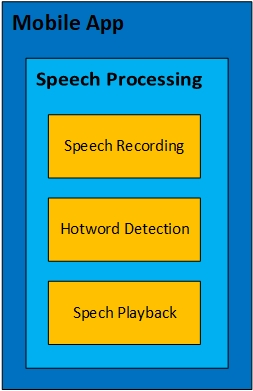
\includegraphics[width=0.3\linewidth]{Picture/Infrastruktur-App.jpg}
	\caption[Architektur - Mobile App]{Architektur - Mobile App}
	\label{fig:infrastruktur-app}
\end{figure}

\subsection{Repository}
Das Repository ist in Abbildung \ref{fig:infrastruktur-repository} dargestellt und unterteilt sich nochmals in zwei Module: Das Runtime Repository und das App Repository, welche im folgenden genauer beschrieben werden.

\begin{itemize}
	\item \textsl{Runtime Repository:} Das Runtime Repository stellt eine Laufzeitumgebung für die Cloud bereit. Die Laufzeitumgebung beinhaltet das Betriebssystem und alle vom Sprachassistenten benötigten Pakete und wird in verschieden Formaten bereitgestellt. Ein Nutzer kann eine Laufzeitumgebung im Format seiner Wahl herunterladen und auf seiner privaten Cloud installieren. Dabei soll die Installation möglichst wenig Konfigurationsaufwand erfordern, denn auch Nutzer ohne IT-Background sollen sich diese Umgebungen installieren können. 
	\item \textsl{App Repository:} Das App Repository stellt alle Apps bereit, die für den Sprachassistenten verfügbar sind. Will ein Nutzer ein App nutzen, so muss er diese in seiner Laufzeitumgebung installieren. Entwickler können Apps im App Repository für Nutzer bereitstellen. Jedoch müssen diese exakte Angaben über die Nutzung der Daten eines Nutzers tätigen. Des Weiteren wird vor einer Veröffentlichung einer App geprüft, ob die Angaben zum Datenschutz korrekt sind und ob diese erfassten Daten überhaupt für die Verbesserung der Nutzerfreundlichkeit notwendig sind. Somit lässt sich Datensparsamkeit für eine App erreichen.
\end{itemize}


\begin{figure}[h!]
	\centering
	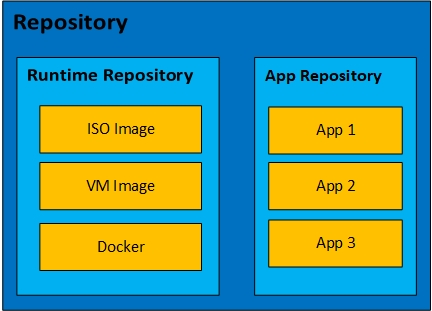
\includegraphics[width=0.6\linewidth]{Picture/Infrastruktur-Repository.jpg}
	\caption[Architektur - Mobile App]{Architektur - Repository}
	\label{fig:infrastruktur-repository}
\end{figure}

\subsection{Laufzeitumgebung}
Die Laufzeitumgebung ist das Herzstück des Sprachassistenten und ist in Abbildung \ref{fig:infrastruktur-cloud} aufgezeigt. Sie beinhaltet einen großen Umfang an Funktionen.

\begin{figure}[h!]
	\centering
	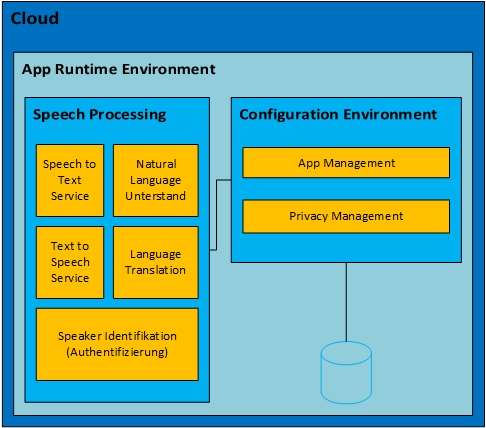
\includegraphics[width=0.9\linewidth]{Picture/Infrastruktur-Cloud.jpg}
	\caption[Architektur - Mobile App]{Architektur - Cloud}
	\label{fig:infrastruktur-cloud}
\end{figure}

\begin{itemize}
	\item \textsl{Sprachverarbeitung:} Das Modul Speech Processing beinhaltet rechenintensive Funktionen der Sprachverarbeitung. Folgende Teilgebiete der Sprachverarbeitung werden für den Sprachassistenten benötigt:
	\begin{itemize}
		\item \textsl{\ac{stt}:} \ac{stt} ist die Umwandlung eines Sprachsignals zu Text.
		\item \textsl{\ac{tts}:} \ac{tts} ist die Umwandlung eines Text zu einem Sprachsignal.
		\item \textsl{\ac{nlu}:} \ac{nlu} ist das Verständnis der natürlichen Sprache. Dies ist nötig, um die Eingabe eines Nutzers zu verstehen. Es kann beispielsweise erkannt werden, ob ein Wort in einem Satz ein Nomen oder Verb ist. 
		\item \textsl{Language Translation:} Hierbei geht es um die Übersetzung eines Texts in eine andere Sprache. Damit kann ein Nutzer mit Nutzern, die eine andere Sprache sprechen kommunizieren. Eine App für den Sprachassistenten kann nicht in der Sprache des Nutzer zur Verfügung stehen, jedoch können die Inhalte der App zur Laufzeit in die Sprache des Nutzers übersetzt werden. Dies minimiert den Entwicklungsaufwand von Apps und erlaubt gleichzeitig das Erreichen einer große Zielgruppe an Nutzern, welche unterschiedlichste Sprachen sprechen. 
		\item \textsl{Speaker Identifikation:} Die Sprecheridentifikation kann als Authentifizierungsmethode des Sprachassistenten dienen. Durch die Sprachinformation in einem Sprachsignal eines Nutzers kann dieser identifiziert werden. Somit kann geprüft werden, ob ein Nutzer die Berechtigung hat, diesen Sprachassistenten zu nutzen.
	\end{itemize}
	\item \textsl{Konfigurationsumgebung:} Über die Konfigurationsumgebung lassen sich die Apps- und Privatsphäre-Einstellungen für den Sprachassistenten vornehmen.
	\begin{itemize}
		\item App Management: Dieses Modul verwaltet die vom Nutzer installierten Apps. Dabei können neue Apps aus dem App Repository installiert oder vorhandene Apps deinstalliert werden.
		\item Privacy Management: Dieses Modul verwaltet den Kontext des Nutzers und erlaubt diesem, den Zugriff von Apps auf diesen Kontext festzulegen. Dabei kann bestimmt werden, welche Informationen des Nutzer von einer App zugänglich sind. Des Weiteren lassen sich auch fiktive Kontexte erstellen, sodass der Nutzer ohne Preisgabe seines tatsächlichen Kontexts eine App nutzen kann. Durch dieses Modul kann User-Controlled-Privacy erreicht werden. 
	\end{itemize}	
\end{itemize}





